\documentclass[twoside]{book}

% Packages required by doxygen
\usepackage{fixltx2e}
\usepackage{calc}
\usepackage{doxygen}
\usepackage[export]{adjustbox} % also loads graphicx
\usepackage{graphicx}
\usepackage[utf8]{inputenc}
\usepackage{makeidx}
\usepackage{multicol}
\usepackage{multirow}
\PassOptionsToPackage{warn}{textcomp}
\usepackage{textcomp}
\usepackage[nointegrals]{wasysym}
\usepackage[table]{xcolor}

% Font selection
\usepackage[T1]{fontenc}
\usepackage[scaled=.90]{helvet}
\usepackage{courier}
\usepackage{amssymb}
\usepackage{sectsty}
\renewcommand{\familydefault}{\sfdefault}
\allsectionsfont{%
  \fontseries{bc}\selectfont%
  \color{darkgray}%
}
\renewcommand{\DoxyLabelFont}{%
  \fontseries{bc}\selectfont%
  \color{darkgray}%
}
\newcommand{\+}{\discretionary{\mbox{\scriptsize$\hookleftarrow$}}{}{}}

% Page & text layout
\usepackage{geometry}
\geometry{%
  a4paper,%
  top=2.5cm,%
  bottom=2.5cm,%
  left=2.5cm,%
  right=2.5cm%
}
\tolerance=750
\hfuzz=15pt
\hbadness=750
\setlength{\emergencystretch}{15pt}
\setlength{\parindent}{0cm}
\setlength{\parskip}{3ex plus 2ex minus 2ex}
\makeatletter
\renewcommand{\paragraph}{%
  \@startsection{paragraph}{4}{0ex}{-1.0ex}{1.0ex}{%
    \normalfont\normalsize\bfseries\SS@parafont%
  }%
}
\renewcommand{\subparagraph}{%
  \@startsection{subparagraph}{5}{0ex}{-1.0ex}{1.0ex}{%
    \normalfont\normalsize\bfseries\SS@subparafont%
  }%
}
\makeatother

% Headers & footers
\usepackage{fancyhdr}
\pagestyle{fancyplain}
\fancyhead[LE]{\fancyplain{}{\bfseries\thepage}}
\fancyhead[CE]{\fancyplain{}{}}
\fancyhead[RE]{\fancyplain{}{\bfseries\leftmark}}
\fancyhead[LO]{\fancyplain{}{\bfseries\rightmark}}
\fancyhead[CO]{\fancyplain{}{}}
\fancyhead[RO]{\fancyplain{}{\bfseries\thepage}}
\fancyfoot[LE]{\fancyplain{}{}}
\fancyfoot[CE]{\fancyplain{}{}}
\fancyfoot[RE]{\fancyplain{}{\bfseries\scriptsize Generated by Doxygen }}
\fancyfoot[LO]{\fancyplain{}{\bfseries\scriptsize Generated by Doxygen }}
\fancyfoot[CO]{\fancyplain{}{}}
\fancyfoot[RO]{\fancyplain{}{}}
\renewcommand{\footrulewidth}{0.4pt}
\renewcommand{\chaptermark}[1]{%
  \markboth{#1}{}%
}
\renewcommand{\sectionmark}[1]{%
  \markright{\thesection\ #1}%
}

% Indices & bibliography
\usepackage{natbib}
\usepackage[titles]{tocloft}
\setcounter{tocdepth}{3}
\setcounter{secnumdepth}{5}
\makeindex

% Hyperlinks (required, but should be loaded last)
\usepackage{ifpdf}
\ifpdf
  \usepackage[pdftex,pagebackref=true]{hyperref}
\else
  \usepackage[ps2pdf,pagebackref=true]{hyperref}
\fi
\hypersetup{%
  colorlinks=true,%
  linkcolor=blue,%
  citecolor=blue,%
  unicode%
}

% Custom commands
\newcommand{\clearemptydoublepage}{%
  \newpage{\pagestyle{empty}\cleardoublepage}%
}

\usepackage{caption}
\captionsetup{labelsep=space,justification=centering,font={bf},singlelinecheck=off,skip=4pt,position=top}

%===== C O N T E N T S =====

\begin{document}

% Titlepage & ToC
\hypersetup{pageanchor=false,
             bookmarksnumbered=true,
             pdfencoding=unicode
            }
\pagenumbering{roman}
\begin{titlepage}
\vspace*{7cm}
\begin{center}%
{\Large My Project }\\
\vspace*{1cm}
{\large Generated by Doxygen 1.8.11}\\
\end{center}
\end{titlepage}
\clearemptydoublepage
\tableofcontents
\clearemptydoublepage
\pagenumbering{arabic}
\hypersetup{pageanchor=true}

%--- Begin generated contents ---
\chapter{Class Index}
\section{Class List}
Here are the classes, structs, unions and interfaces with brief descriptions\+:\begin{DoxyCompactList}
\item\contentsline{section}{\hyperlink{structnode}{node} }{\pageref{structnode}}{}
\item\contentsline{section}{\hyperlink{structnode1}{node1} }{\pageref{structnode1}}{}
\item\contentsline{section}{\hyperlink{structnode__info}{node\+\_\+info} }{\pageref{structnode__info}}{}
\end{DoxyCompactList}

\chapter{File Index}
\section{File List}
Here is a list of all files with brief descriptions\+:\begin{DoxyCompactList}
\item\contentsline{section}{\hyperlink{Lab1_8c}{Lab1.\+c} }{\pageref{Lab1_8c}}{}
\end{DoxyCompactList}

\chapter{Class Documentation}
\hypertarget{structnode}{}\section{node Struct Reference}
\label{structnode}\index{node@{node}}


Collaboration diagram for node\+:
\nopagebreak
\begin{figure}[H]
\begin{center}
\leavevmode
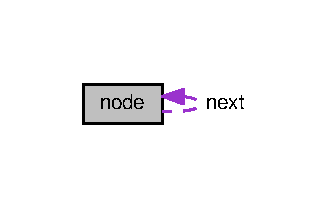
\includegraphics[width=158pt]{structnode__coll__graph}
\end{center}
\end{figure}
\subsection*{Public Attributes}
\begin{DoxyCompactItemize}
\item 
int \hyperlink{structnode_a2d890bb9f6af0ffd73fe79b21124c2a2}{data}
\item 
\hyperlink{structnode}{node} $\ast$ \hyperlink{structnode_aad210fa7c160a49f6b9a3ffee592a2bc}{next}
\end{DoxyCompactItemize}


\subsection{Member Data Documentation}
\index{node@{node}!data@{data}}
\index{data@{data}!node@{node}}
\subsubsection[{\texorpdfstring{data}{data}}]{\setlength{\rightskip}{0pt plus 5cm}int node\+::data}\hypertarget{structnode_a2d890bb9f6af0ffd73fe79b21124c2a2}{}\label{structnode_a2d890bb9f6af0ffd73fe79b21124c2a2}
\index{node@{node}!next@{next}}
\index{next@{next}!node@{node}}
\subsubsection[{\texorpdfstring{next}{next}}]{\setlength{\rightskip}{0pt plus 5cm}{\bf node}$\ast$ node\+::next}\hypertarget{structnode_aad210fa7c160a49f6b9a3ffee592a2bc}{}\label{structnode_aad210fa7c160a49f6b9a3ffee592a2bc}


The documentation for this struct was generated from the following file\+:\begin{DoxyCompactItemize}
\item 
\hyperlink{SelfOrganizing_8cpp}{Self\+Organizing.\+cpp}\end{DoxyCompactItemize}

\hypertarget{structqueue}{}\section{queue Struct Reference}
\label{structqueue}\index{queue@{queue}}


{\ttfamily \#include $<$List\+Students\+\_\+queue.\+h$>$}



Collaboration diagram for queue\+:
\nopagebreak
\begin{figure}[H]
\begin{center}
\leavevmode
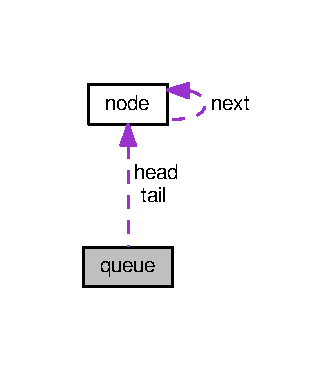
\includegraphics[width=161pt]{structqueue__coll__graph}
\end{center}
\end{figure}
\subsection*{Public Attributes}
\begin{DoxyCompactItemize}
\item 
int \hyperlink{structqueue_a652887eeb98c5e87bed0662c2da0e723}{nodesize}
\item 
\hyperlink{ListStudents__queue_8h_a0bfdc21bc19acf8a0ac274ebd1b6304a}{nodeptr} \hyperlink{structqueue_a23e9f810057d92adf24e3278dfe7865f}{head}
\item 
\hyperlink{ListStudents__queue_8h_a0bfdc21bc19acf8a0ac274ebd1b6304a}{nodeptr} \hyperlink{structqueue_a827de955c3490873a13e63e5478b444b}{tail}
\end{DoxyCompactItemize}


\subsection{Member Data Documentation}
\index{queue@{queue}!head@{head}}
\index{head@{head}!queue@{queue}}
\subsubsection[{\texorpdfstring{head}{head}}]{\setlength{\rightskip}{0pt plus 5cm}{\bf nodeptr} queue\+::head}\hypertarget{structqueue_a23e9f810057d92adf24e3278dfe7865f}{}\label{structqueue_a23e9f810057d92adf24e3278dfe7865f}
\index{queue@{queue}!nodesize@{nodesize}}
\index{nodesize@{nodesize}!queue@{queue}}
\subsubsection[{\texorpdfstring{nodesize}{nodesize}}]{\setlength{\rightskip}{0pt plus 5cm}int queue\+::nodesize}\hypertarget{structqueue_a652887eeb98c5e87bed0662c2da0e723}{}\label{structqueue_a652887eeb98c5e87bed0662c2da0e723}
\index{queue@{queue}!tail@{tail}}
\index{tail@{tail}!queue@{queue}}
\subsubsection[{\texorpdfstring{tail}{tail}}]{\setlength{\rightskip}{0pt plus 5cm}{\bf nodeptr} queue\+::tail}\hypertarget{structqueue_a827de955c3490873a13e63e5478b444b}{}\label{structqueue_a827de955c3490873a13e63e5478b444b}


The documentation for this struct was generated from the following file\+:\begin{DoxyCompactItemize}
\item 
\hyperlink{ListStudents__queue_8h}{List\+Students\+\_\+queue.\+h}\end{DoxyCompactItemize}

\hypertarget{structstudent}{}\section{student Struct Reference}
\label{structstudent}\index{student@{student}}
\subsection*{Public Attributes}
\begin{DoxyCompactItemize}
\item 
char \hyperlink{structstudent_a4cc31cdf611c0cce37bba9239ea27ae3}{name} \mbox{[}\hyperlink{ListStudents__main_8c_ad79aefee6a8990632311a15e98d9a65f}{N\+A\+M\+E\+S\+I\+ZE}\mbox{]}
\item 
int \hyperlink{structstudent_a0044e7dfdd90788897b708b0a64af0ee}{midterm}
\item 
int \hyperlink{structstudent_a4a15ad9d47eea21ab8b157561f01f2a4}{final}
\item 
int \hyperlink{structstudent_aa02b98056cfb79a6a5012667be2e717b}{homeworks}
\end{DoxyCompactItemize}


\subsection{Member Data Documentation}
\index{student@{student}!final@{final}}
\index{final@{final}!student@{student}}
\subsubsection[{\texorpdfstring{final}{final}}]{\setlength{\rightskip}{0pt plus 5cm}int student\+::final}\hypertarget{structstudent_a4a15ad9d47eea21ab8b157561f01f2a4}{}\label{structstudent_a4a15ad9d47eea21ab8b157561f01f2a4}
\index{student@{student}!homeworks@{homeworks}}
\index{homeworks@{homeworks}!student@{student}}
\subsubsection[{\texorpdfstring{homeworks}{homeworks}}]{\setlength{\rightskip}{0pt plus 5cm}int student\+::homeworks}\hypertarget{structstudent_aa02b98056cfb79a6a5012667be2e717b}{}\label{structstudent_aa02b98056cfb79a6a5012667be2e717b}
\index{student@{student}!midterm@{midterm}}
\index{midterm@{midterm}!student@{student}}
\subsubsection[{\texorpdfstring{midterm}{midterm}}]{\setlength{\rightskip}{0pt plus 5cm}int student\+::midterm}\hypertarget{structstudent_a0044e7dfdd90788897b708b0a64af0ee}{}\label{structstudent_a0044e7dfdd90788897b708b0a64af0ee}
\index{student@{student}!name@{name}}
\index{name@{name}!student@{student}}
\subsubsection[{\texorpdfstring{name}{name}}]{\setlength{\rightskip}{0pt plus 5cm}char student\+::name\mbox{[}{\bf N\+A\+M\+E\+S\+I\+ZE}\mbox{]}}\hypertarget{structstudent_a4cc31cdf611c0cce37bba9239ea27ae3}{}\label{structstudent_a4cc31cdf611c0cce37bba9239ea27ae3}


The documentation for this struct was generated from the following file\+:\begin{DoxyCompactItemize}
\item 
\hyperlink{ListStudents__main_8c}{List\+Students\+\_\+main.\+c}\end{DoxyCompactItemize}

\chapter{File Documentation}
\hypertarget{ListStudents__main_8c}{}\section{List\+Students\+\_\+main.\+c File Reference}
\label{ListStudents__main_8c}\index{List\+Students\+\_\+main.\+c@{List\+Students\+\_\+main.\+c}}
{\ttfamily \#include $<$stdio.\+h$>$}\\*
{\ttfamily \#include \char`\"{}List\+Students\+\_\+queue.\+h\char`\"{}}\\*
Include dependency graph for List\+Students\+\_\+main.\+c\+:
\nopagebreak
\begin{figure}[H]
\begin{center}
\leavevmode
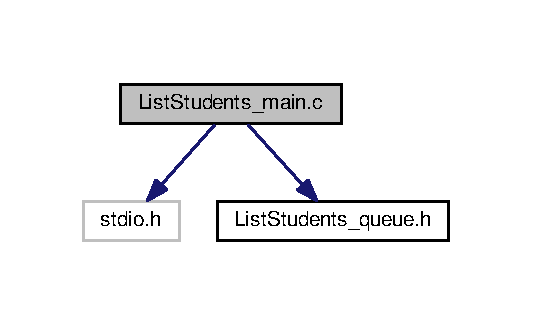
\includegraphics[width=256pt]{ListStudents__main_8c__incl}
\end{center}
\end{figure}
\subsection*{Classes}
\begin{DoxyCompactItemize}
\item 
struct \hyperlink{structstudent}{student}
\end{DoxyCompactItemize}
\subsection*{Macros}
\begin{DoxyCompactItemize}
\item 
\#define \hyperlink{ListStudents__main_8c_ad79aefee6a8990632311a15e98d9a65f}{N\+A\+M\+E\+S\+I\+ZE}~25
\end{DoxyCompactItemize}
\subsection*{Typedefs}
\begin{DoxyCompactItemize}
\item 
typedef \hyperlink{structstudent}{student} $\ast$ \hyperlink{ListStudents__main_8c_a0b11d0a1e6f1f884c7ee456c297762db}{studentptr}
\end{DoxyCompactItemize}
\subsection*{Functions}
\begin{DoxyCompactItemize}
\item 
void \hyperlink{ListStudents__main_8c_a1b41f1bf22121a8616fa316bfa258262}{write\+Student\+List} (char filename\mbox{[}$\,$\mbox{]}, \hyperlink{structqueue}{queue} $\ast$q)
\item 
int \hyperlink{ListStudents__main_8c_a06ff31ab1d0e694ba9c35eb08e583950}{read\+Student\+List} (char filename\mbox{[}$\,$\mbox{]}, \hyperlink{structqueue}{queue} $\ast$q)
\item 
int \hyperlink{ListStudents__main_8c_a0ddf1224851353fc92bfbff6f499fa97}{main} (int argc, char $\ast$argv\mbox{[}$\,$\mbox{]})
\end{DoxyCompactItemize}


\subsection{Macro Definition Documentation}
\index{List\+Students\+\_\+main.\+c@{List\+Students\+\_\+main.\+c}!N\+A\+M\+E\+S\+I\+ZE@{N\+A\+M\+E\+S\+I\+ZE}}
\index{N\+A\+M\+E\+S\+I\+ZE@{N\+A\+M\+E\+S\+I\+ZE}!List\+Students\+\_\+main.\+c@{List\+Students\+\_\+main.\+c}}
\subsubsection[{\texorpdfstring{N\+A\+M\+E\+S\+I\+ZE}{NAMESIZE}}]{\setlength{\rightskip}{0pt plus 5cm}\#define N\+A\+M\+E\+S\+I\+ZE~25}\hypertarget{ListStudents__main_8c_ad79aefee6a8990632311a15e98d9a65f}{}\label{ListStudents__main_8c_ad79aefee6a8990632311a15e98d9a65f}


\subsection{Typedef Documentation}
\index{List\+Students\+\_\+main.\+c@{List\+Students\+\_\+main.\+c}!studentptr@{studentptr}}
\index{studentptr@{studentptr}!List\+Students\+\_\+main.\+c@{List\+Students\+\_\+main.\+c}}
\subsubsection[{\texorpdfstring{studentptr}{studentptr}}]{\setlength{\rightskip}{0pt plus 5cm}typedef {\bf student}$\ast$ {\bf studentptr}}\hypertarget{ListStudents__main_8c_a0b11d0a1e6f1f884c7ee456c297762db}{}\label{ListStudents__main_8c_a0b11d0a1e6f1f884c7ee456c297762db}


\subsection{Function Documentation}
\index{List\+Students\+\_\+main.\+c@{List\+Students\+\_\+main.\+c}!main@{main}}
\index{main@{main}!List\+Students\+\_\+main.\+c@{List\+Students\+\_\+main.\+c}}
\subsubsection[{\texorpdfstring{main(int argc, char $\ast$argv[])}{main(int argc, char *argv[])}}]{\setlength{\rightskip}{0pt plus 5cm}int main (
\begin{DoxyParamCaption}
\item[{int}]{argc, }
\item[{char $\ast$}]{argv\mbox{[}$\,$\mbox{]}}
\end{DoxyParamCaption}
)}\hypertarget{ListStudents__main_8c_a0ddf1224851353fc92bfbff6f499fa97}{}\label{ListStudents__main_8c_a0ddf1224851353fc92bfbff6f499fa97}

\begin{DoxyCode}
71                                 \{
72   \textcolor{keywordtype}{int} n;
73   \hyperlink{structqueue}{queue} *q;
74 
75   \textcolor{keywordflow}{if}(argc!=3)\{
76     printf(\textcolor{stringliteral}{"Usage: %s infile outfile\(\backslash\)n"}, argv[0]);
77     exit(0);
78   \}
79   q = \hyperlink{ListStudents__queue_8c_a224704b6af1ea85c374ee7bed6a80b41}{init}(\textcolor{keyword}{sizeof}(\hyperlink{structstudent}{student}));
80   n = \hyperlink{ListStudents__main_8c_a06ff31ab1d0e694ba9c35eb08e583950}{readStudentList}(argv[1],q);
81   \hyperlink{ListStudents__main_8c_a1b41f1bf22121a8616fa316bfa258262}{writeStudentList}(argv[2],q);
82   \textcolor{keyword}{final}(q);
83 \}
\end{DoxyCode}


Here is the call graph for this function\+:
\nopagebreak
\begin{figure}[H]
\begin{center}
\leavevmode
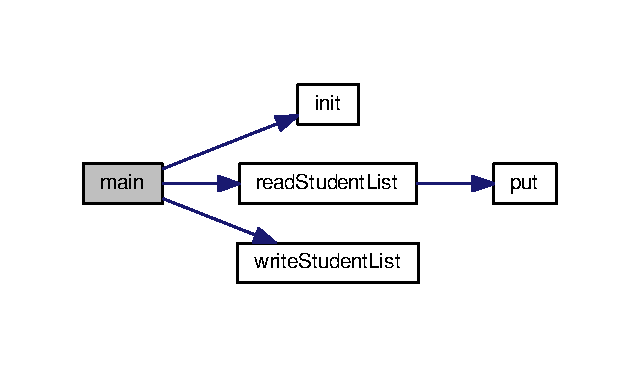
\includegraphics[width=307pt]{ListStudents__main_8c_a0ddf1224851353fc92bfbff6f499fa97_cgraph}
\end{center}
\end{figure}


\index{List\+Students\+\_\+main.\+c@{List\+Students\+\_\+main.\+c}!read\+Student\+List@{read\+Student\+List}}
\index{read\+Student\+List@{read\+Student\+List}!List\+Students\+\_\+main.\+c@{List\+Students\+\_\+main.\+c}}
\subsubsection[{\texorpdfstring{read\+Student\+List(char filename[], queue $\ast$q)}{readStudentList(char filename[], queue *q)}}]{\setlength{\rightskip}{0pt plus 5cm}int read\+Student\+List (
\begin{DoxyParamCaption}
\item[{char}]{filename\mbox{[}$\,$\mbox{]}, }
\item[{{\bf queue} $\ast$}]{q}
\end{DoxyParamCaption}
)}\hypertarget{ListStudents__main_8c_a06ff31ab1d0e694ba9c35eb08e583950}{}\label{ListStudents__main_8c_a06ff31ab1d0e694ba9c35eb08e583950}

\begin{DoxyCode}
50 \{
51   FILE *fd;  \textcolor{comment}{/* File descriptor used for filename */}
52   \textcolor{keywordtype}{int} i=0;
53   \hyperlink{structstudent}{student} temp;
54   
55   \textcolor{keywordflow}{if}((fd=fopen(filename,\textcolor{stringliteral}{"r"}))==NULL)\{
56     perror(\textcolor{stringliteral}{"fopen"});
57     exit(1);
58   \}
59   \textcolor{keywordflow}{while}(fscanf(fd,\textcolor{stringliteral}{"%s %d %d %d"},
60            temp.\hyperlink{structstudent_a4cc31cdf611c0cce37bba9239ea27ae3}{name}, 
61            &temp.\hyperlink{structstudent_a0044e7dfdd90788897b708b0a64af0ee}{midterm},
62            &temp.\hyperlink{structstudent_a4a15ad9d47eea21ab8b157561f01f2a4}{final}, 
63            &temp.\hyperlink{structstudent_aa02b98056cfb79a6a5012667be2e717b}{homeworks})!=EOF)\{
64     \hyperlink{ListStudents__queue_8c_ab88e40b482be2c89256c133fad50ec89}{put}(q,&temp);
65     i++;
66   \}
67   fclose(fd);
68   \textcolor{keywordflow}{return} i;
69 \}
\end{DoxyCode}


Here is the call graph for this function\+:
\nopagebreak
\begin{figure}[H]
\begin{center}
\leavevmode
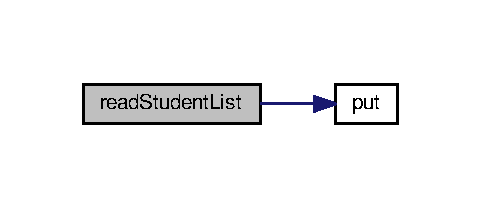
\includegraphics[width=231pt]{ListStudents__main_8c_a06ff31ab1d0e694ba9c35eb08e583950_cgraph}
\end{center}
\end{figure}


\index{List\+Students\+\_\+main.\+c@{List\+Students\+\_\+main.\+c}!write\+Student\+List@{write\+Student\+List}}
\index{write\+Student\+List@{write\+Student\+List}!List\+Students\+\_\+main.\+c@{List\+Students\+\_\+main.\+c}}
\subsubsection[{\texorpdfstring{write\+Student\+List(char filename[], queue $\ast$q)}{writeStudentList(char filename[], queue *q)}}]{\setlength{\rightskip}{0pt plus 5cm}void write\+Student\+List (
\begin{DoxyParamCaption}
\item[{char}]{filename\mbox{[}$\,$\mbox{]}, }
\item[{{\bf queue} $\ast$}]{q}
\end{DoxyParamCaption}
)}\hypertarget{ListStudents__main_8c_a1b41f1bf22121a8616fa316bfa258262}{}\label{ListStudents__main_8c_a1b41f1bf22121a8616fa316bfa258262}

\begin{DoxyCode}
27 \{
28   FILE *fd;  \textcolor{comment}{/* File descriptor used for filename */}
29   \hyperlink{structstudent}{studentptr} s;
30 
31   \textcolor{keywordflow}{if}((fd=fopen(filename,\textcolor{stringliteral}{"w"}))==NULL)\{
32     perror(\textcolor{stringliteral}{"fopen"});
33     exit(1);
34   \}
35   \textcolor{keywordflow}{while}(\textcolor{keyword}{get}(q, s))\{
36     fprintf(fd,\textcolor{stringliteral}{"%s %d %d %d\(\backslash\)n"},
37         s->\hyperlink{structstudent_a4cc31cdf611c0cce37bba9239ea27ae3}{name}, 
38         s->\hyperlink{structstudent_a0044e7dfdd90788897b708b0a64af0ee}{midterm}, 
39         s->\hyperlink{structstudent_a4a15ad9d47eea21ab8b157561f01f2a4}{final}, 
40         s->\hyperlink{structstudent_aa02b98056cfb79a6a5012667be2e717b}{homeworks});
41   \}
42   fclose(fd);
43 \}
\end{DoxyCode}

\hypertarget{ListStudents__queue_8c}{}\section{List\+Students\+\_\+queue.\+c File Reference}
\label{ListStudents__queue_8c}\index{List\+Students\+\_\+queue.\+c@{List\+Students\+\_\+queue.\+c}}
{\ttfamily \#include $<$stdio.\+h$>$}\\*
{\ttfamily \#include $<$stdlib.\+h$>$}\\*
{\ttfamily \#include \char`\"{}List\+Students\+\_\+queue.\+h\char`\"{}}\\*
Include dependency graph for List\+Students\+\_\+queue.\+c\+:
\nopagebreak
\begin{figure}[H]
\begin{center}
\leavevmode
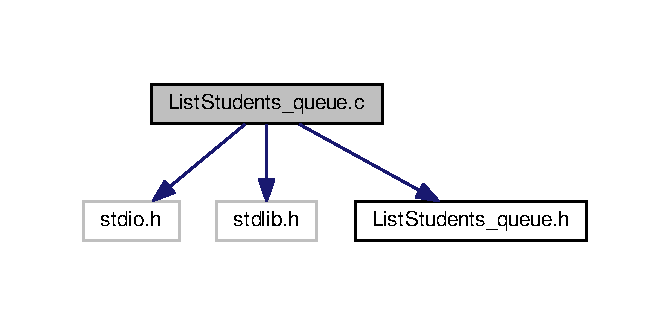
\includegraphics[width=322pt]{ListStudents__queue_8c__incl}
\end{center}
\end{figure}
\subsection*{Functions}
\begin{DoxyCompactItemize}
\item 
\hyperlink{structqueue}{queue} $\ast$ \hyperlink{ListStudents__queue_8c_a224704b6af1ea85c374ee7bed6a80b41}{init} (int n)
\item 
void \hyperlink{ListStudents__queue_8c_a14b9ca3a8fda3effd9ef8ad947119c3b}{final} (\hyperlink{structqueue}{queue} $\ast$q)
\item 
void \hyperlink{ListStudents__queue_8c_ab88e40b482be2c89256c133fad50ec89}{put} (\hyperlink{structqueue}{queue} $\ast$q, void $\ast$s)
\item 
int \hyperlink{ListStudents__queue_8c_ae086d7328a275c2ee8b01943a82172dc}{get} (\hyperlink{structqueue}{queue} $\ast$q, void $\ast$s)
\end{DoxyCompactItemize}


\subsection{Function Documentation}
\index{List\+Students\+\_\+queue.\+c@{List\+Students\+\_\+queue.\+c}!final@{final}}
\index{final@{final}!List\+Students\+\_\+queue.\+c@{List\+Students\+\_\+queue.\+c}}
\subsubsection[{\texorpdfstring{final(queue $\ast$q)}{final(queue *q)}}]{\setlength{\rightskip}{0pt plus 5cm}void final (
\begin{DoxyParamCaption}
\item[{{\bf queue} $\ast$}]{q}
\end{DoxyParamCaption}
)}\hypertarget{ListStudents__queue_8c_a14b9ca3a8fda3effd9ef8ad947119c3b}{}\label{ListStudents__queue_8c_a14b9ca3a8fda3effd9ef8ad947119c3b}

\begin{DoxyCode}
23                     \{
24   \textcolor{comment}{/* It frees all storage associated with the queue q */}
25   \textcolor{keywordtype}{char} *s;
26 
27   \textcolor{keywordflow}{if}((s=(\textcolor{keywordtype}{char} *)malloc(q->\hyperlink{structqueue_a652887eeb98c5e87bed0662c2da0e723}{nodesize}))==NULL)\{
28     perror(\textcolor{stringliteral}{"malloc"});
29     exit(1);
30   \}
31   \textcolor{keywordflow}{while}(\textcolor{keyword}{get}(q,s));
32   free(q);
33   free(s);
34 \}
\end{DoxyCode}
\index{List\+Students\+\_\+queue.\+c@{List\+Students\+\_\+queue.\+c}!get@{get}}
\index{get@{get}!List\+Students\+\_\+queue.\+c@{List\+Students\+\_\+queue.\+c}}
\subsubsection[{\texorpdfstring{get(queue $\ast$q, void $\ast$s)}{get(queue *q, void *s)}}]{\setlength{\rightskip}{0pt plus 5cm}int get (
\begin{DoxyParamCaption}
\item[{{\bf queue} $\ast$}]{q, }
\item[{void $\ast$}]{s}
\end{DoxyParamCaption}
)}\hypertarget{ListStudents__queue_8c_ae086d7328a275c2ee8b01943a82172dc}{}\label{ListStudents__queue_8c_ae086d7328a275c2ee8b01943a82172dc}

\begin{DoxyCode}
59                           \{
60   \textcolor{comment}{/*It obtains in *s a copy of a value from queue q. It returns true
}
61 \textcolor{comment}{    iff such a record existed */}
62   \hyperlink{structnode}{nodeptr} p;
63 
64   \textcolor{keywordflow}{if}(p=q->\hyperlink{structqueue_a23e9f810057d92adf24e3278dfe7865f}{head})\{
65     q->\hyperlink{structqueue_a23e9f810057d92adf24e3278dfe7865f}{head} = q->\hyperlink{structqueue_a23e9f810057d92adf24e3278dfe7865f}{head}->\hyperlink{structnode_aa3e8aa83f864292b5a01210f4453fcc0}{next};
66     \textcolor{keywordflow}{if}((q->\hyperlink{structqueue_a23e9f810057d92adf24e3278dfe7865f}{head})==NULL)
67       q->\hyperlink{structqueue_a827de955c3490873a13e63e5478b444b}{tail} = NULL;
68     bcopy(p->\hyperlink{structnode_a288a44aecd04d7839824d50a0b65982e}{value},s,q->\hyperlink{structqueue_a652887eeb98c5e87bed0662c2da0e723}{nodesize});
69     free(p->\hyperlink{structnode_a288a44aecd04d7839824d50a0b65982e}{value});
70     free(p);
71     \textcolor{keywordflow}{return} 1;
72   \}\textcolor{keywordflow}{else}
73     \textcolor{keywordflow}{return} 0;
74 \}
\end{DoxyCode}
\index{List\+Students\+\_\+queue.\+c@{List\+Students\+\_\+queue.\+c}!init@{init}}
\index{init@{init}!List\+Students\+\_\+queue.\+c@{List\+Students\+\_\+queue.\+c}}
\subsubsection[{\texorpdfstring{init(int n)}{init(int n)}}]{\setlength{\rightskip}{0pt plus 5cm}{\bf queue}$\ast$ init (
\begin{DoxyParamCaption}
\item[{int}]{n}
\end{DoxyParamCaption}
)}\hypertarget{ListStudents__queue_8c_a224704b6af1ea85c374ee7bed6a80b41}{}\label{ListStudents__queue_8c_a224704b6af1ea85c374ee7bed6a80b41}

\begin{DoxyCode}
8                   \{
9   \textcolor{comment}{/* It creates, initializes, and returns a queue that stores values
}
10 \textcolor{comment}{     of size n */}
11   \hyperlink{structqueue}{queue} *q;
12 
13   \textcolor{keywordflow}{if}((q=(\hyperlink{structqueue}{queue} *)malloc(\textcolor{keyword}{sizeof}(\hyperlink{structqueue}{queue})))==NULL)\{
14     perror(\textcolor{stringliteral}{"malloc"});
15     exit(1);
16   \}
17   q->\hyperlink{structqueue_a652887eeb98c5e87bed0662c2da0e723}{nodesize}=n;
18   q->\hyperlink{structqueue_a23e9f810057d92adf24e3278dfe7865f}{head}=NULL;
19   q->\hyperlink{structqueue_a827de955c3490873a13e63e5478b444b}{tail}=NULL;
20   \textcolor{keywordflow}{return} q;
21 \}
\end{DoxyCode}
\index{List\+Students\+\_\+queue.\+c@{List\+Students\+\_\+queue.\+c}!put@{put}}
\index{put@{put}!List\+Students\+\_\+queue.\+c@{List\+Students\+\_\+queue.\+c}}
\subsubsection[{\texorpdfstring{put(queue $\ast$q, void $\ast$s)}{put(queue *q, void *s)}}]{\setlength{\rightskip}{0pt plus 5cm}void put (
\begin{DoxyParamCaption}
\item[{{\bf queue} $\ast$}]{q, }
\item[{void $\ast$}]{s}
\end{DoxyParamCaption}
)}\hypertarget{ListStudents__queue_8c_ab88e40b482be2c89256c133fad50ec89}{}\label{ListStudents__queue_8c_ab88e40b482be2c89256c133fad50ec89}

\begin{DoxyCode}
36                             \{
37   \textcolor{comment}{/* It inserts a copy of the value *s in the queue q */}
38   \hyperlink{structnode}{nodeptr} p;
39   \textcolor{keywordtype}{void} *r;
40   
41   \textcolor{keywordflow}{if} ((p=(\hyperlink{structnode}{nodeptr})malloc(\textcolor{keyword}{sizeof}(\hyperlink{structnode}{node})))==NULL)\{
42     perror(\textcolor{stringliteral}{"malloc"});
43     exit(1);
44   \}
45   \textcolor{keywordflow}{if} ((r=(\textcolor{keywordtype}{void} *)malloc(q->\hyperlink{structqueue_a652887eeb98c5e87bed0662c2da0e723}{nodesize}))==NULL)\{
46     perror(\textcolor{stringliteral}{"malloc"});
47     exit(1);
48   \}
49   bcopy(s,r,q->\hyperlink{structqueue_a652887eeb98c5e87bed0662c2da0e723}{nodesize});
50   p->\hyperlink{structnode_a288a44aecd04d7839824d50a0b65982e}{value} = r;
51   p->\hyperlink{structnode_aa3e8aa83f864292b5a01210f4453fcc0}{next} = NULL;
52   \textcolor{keywordflow}{if} (q->\hyperlink{structqueue_a23e9f810057d92adf24e3278dfe7865f}{head} == NULL)
53     q->\hyperlink{structqueue_a23e9f810057d92adf24e3278dfe7865f}{head} = p;
54   \textcolor{keywordflow}{else}
55     q->\hyperlink{structqueue_a827de955c3490873a13e63e5478b444b}{tail}->\hyperlink{structnode_aa3e8aa83f864292b5a01210f4453fcc0}{next} = p;
56   q->\hyperlink{structqueue_a827de955c3490873a13e63e5478b444b}{tail} = p;
57 \}
\end{DoxyCode}

\hypertarget{ListStudents__queue_8h}{}\section{List\+Students\+\_\+queue.\+h File Reference}
\label{ListStudents__queue_8h}\index{List\+Students\+\_\+queue.\+h@{List\+Students\+\_\+queue.\+h}}
This graph shows which files directly or indirectly include this file\+:
\nopagebreak
\begin{figure}[H]
\begin{center}
\leavevmode
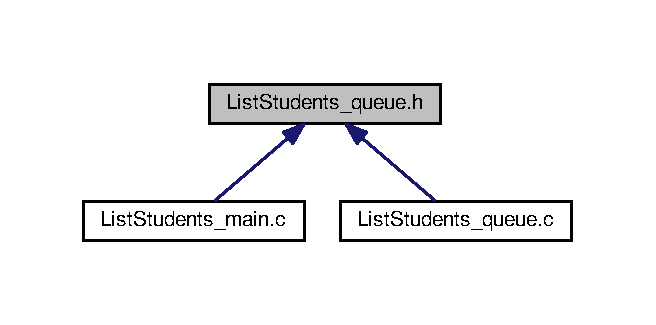
\includegraphics[width=315pt]{ListStudents__queue_8h__dep__incl}
\end{center}
\end{figure}
\subsection*{Classes}
\begin{DoxyCompactItemize}
\item 
struct \hyperlink{structnode}{node}
\item 
struct \hyperlink{structqueue}{queue}
\end{DoxyCompactItemize}
\subsection*{Typedefs}
\begin{DoxyCompactItemize}
\item 
typedef struct \hyperlink{structnode}{node} \hyperlink{ListStudents__queue_8h_af4aeda155dbe167f1c1cf38cb65bf324}{node}
\item 
typedef \hyperlink{structnode}{node} $\ast$ \hyperlink{ListStudents__queue_8h_a0bfdc21bc19acf8a0ac274ebd1b6304a}{nodeptr}
\end{DoxyCompactItemize}
\subsection*{Functions}
\begin{DoxyCompactItemize}
\item 
\hyperlink{structqueue}{queue} $\ast$ \hyperlink{ListStudents__queue_8h_a224704b6af1ea85c374ee7bed6a80b41}{init} (int n)
\item 
void \hyperlink{ListStudents__queue_8h_a14b9ca3a8fda3effd9ef8ad947119c3b}{final} (\hyperlink{structqueue}{queue} $\ast$q)
\item 
void \hyperlink{ListStudents__queue_8h_ab88e40b482be2c89256c133fad50ec89}{put} (\hyperlink{structqueue}{queue} $\ast$q, void $\ast$s)
\item 
int \hyperlink{ListStudents__queue_8h_ae086d7328a275c2ee8b01943a82172dc}{get} (\hyperlink{structqueue}{queue} $\ast$q, void $\ast$s)
\end{DoxyCompactItemize}


\subsection{Typedef Documentation}
\index{List\+Students\+\_\+queue.\+h@{List\+Students\+\_\+queue.\+h}!node@{node}}
\index{node@{node}!List\+Students\+\_\+queue.\+h@{List\+Students\+\_\+queue.\+h}}
\subsubsection[{\texorpdfstring{node}{node}}]{\setlength{\rightskip}{0pt plus 5cm}typedef struct {\bf node} {\bf node}}\hypertarget{ListStudents__queue_8h_af4aeda155dbe167f1c1cf38cb65bf324}{}\label{ListStudents__queue_8h_af4aeda155dbe167f1c1cf38cb65bf324}
\index{List\+Students\+\_\+queue.\+h@{List\+Students\+\_\+queue.\+h}!nodeptr@{nodeptr}}
\index{nodeptr@{nodeptr}!List\+Students\+\_\+queue.\+h@{List\+Students\+\_\+queue.\+h}}
\subsubsection[{\texorpdfstring{nodeptr}{nodeptr}}]{\setlength{\rightskip}{0pt plus 5cm}typedef {\bf node}$\ast$ {\bf nodeptr}}\hypertarget{ListStudents__queue_8h_a0bfdc21bc19acf8a0ac274ebd1b6304a}{}\label{ListStudents__queue_8h_a0bfdc21bc19acf8a0ac274ebd1b6304a}


\subsection{Function Documentation}
\index{List\+Students\+\_\+queue.\+h@{List\+Students\+\_\+queue.\+h}!final@{final}}
\index{final@{final}!List\+Students\+\_\+queue.\+h@{List\+Students\+\_\+queue.\+h}}
\subsubsection[{\texorpdfstring{final(queue $\ast$q)}{final(queue *q)}}]{\setlength{\rightskip}{0pt plus 5cm}void final (
\begin{DoxyParamCaption}
\item[{{\bf queue} $\ast$}]{q}
\end{DoxyParamCaption}
)}\hypertarget{ListStudents__queue_8h_a14b9ca3a8fda3effd9ef8ad947119c3b}{}\label{ListStudents__queue_8h_a14b9ca3a8fda3effd9ef8ad947119c3b}

\begin{DoxyCode}
23                     \{
24   \textcolor{comment}{/* It frees all storage associated with the queue q */}
25   \textcolor{keywordtype}{char} *s;
26 
27   \textcolor{keywordflow}{if}((s=(\textcolor{keywordtype}{char} *)malloc(q->\hyperlink{structqueue_a652887eeb98c5e87bed0662c2da0e723}{nodesize}))==NULL)\{
28     perror(\textcolor{stringliteral}{"malloc"});
29     exit(1);
30   \}
31   \textcolor{keywordflow}{while}(\textcolor{keyword}{get}(q,s));
32   free(q);
33   free(s);
34 \}
\end{DoxyCode}
\index{List\+Students\+\_\+queue.\+h@{List\+Students\+\_\+queue.\+h}!get@{get}}
\index{get@{get}!List\+Students\+\_\+queue.\+h@{List\+Students\+\_\+queue.\+h}}
\subsubsection[{\texorpdfstring{get(queue $\ast$q, void $\ast$s)}{get(queue *q, void *s)}}]{\setlength{\rightskip}{0pt plus 5cm}int get (
\begin{DoxyParamCaption}
\item[{{\bf queue} $\ast$}]{q, }
\item[{void $\ast$}]{s}
\end{DoxyParamCaption}
)}\hypertarget{ListStudents__queue_8h_ae086d7328a275c2ee8b01943a82172dc}{}\label{ListStudents__queue_8h_ae086d7328a275c2ee8b01943a82172dc}

\begin{DoxyCode}
59                           \{
60   \textcolor{comment}{/*It obtains in *s a copy of a value from queue q. It returns true
}
61 \textcolor{comment}{    iff such a record existed */}
62   \hyperlink{structnode}{nodeptr} p;
63 
64   \textcolor{keywordflow}{if}(p=q->\hyperlink{structqueue_a23e9f810057d92adf24e3278dfe7865f}{head})\{
65     q->\hyperlink{structqueue_a23e9f810057d92adf24e3278dfe7865f}{head} = q->\hyperlink{structqueue_a23e9f810057d92adf24e3278dfe7865f}{head}->\hyperlink{structnode_aa3e8aa83f864292b5a01210f4453fcc0}{next};
66     \textcolor{keywordflow}{if}((q->\hyperlink{structqueue_a23e9f810057d92adf24e3278dfe7865f}{head})==NULL)
67       q->\hyperlink{structqueue_a827de955c3490873a13e63e5478b444b}{tail} = NULL;
68     bcopy(p->\hyperlink{structnode_a288a44aecd04d7839824d50a0b65982e}{value},s,q->\hyperlink{structqueue_a652887eeb98c5e87bed0662c2da0e723}{nodesize});
69     free(p->\hyperlink{structnode_a288a44aecd04d7839824d50a0b65982e}{value});
70     free(p);
71     \textcolor{keywordflow}{return} 1;
72   \}\textcolor{keywordflow}{else}
73     \textcolor{keywordflow}{return} 0;
74 \}
\end{DoxyCode}
\index{List\+Students\+\_\+queue.\+h@{List\+Students\+\_\+queue.\+h}!init@{init}}
\index{init@{init}!List\+Students\+\_\+queue.\+h@{List\+Students\+\_\+queue.\+h}}
\subsubsection[{\texorpdfstring{init(int n)}{init(int n)}}]{\setlength{\rightskip}{0pt plus 5cm}{\bf queue}$\ast$ init (
\begin{DoxyParamCaption}
\item[{int}]{n}
\end{DoxyParamCaption}
)}\hypertarget{ListStudents__queue_8h_a224704b6af1ea85c374ee7bed6a80b41}{}\label{ListStudents__queue_8h_a224704b6af1ea85c374ee7bed6a80b41}

\begin{DoxyCode}
8                   \{
9   \textcolor{comment}{/* It creates, initializes, and returns a queue that stores values
}
10 \textcolor{comment}{     of size n */}
11   \hyperlink{structqueue}{queue} *q;
12 
13   \textcolor{keywordflow}{if}((q=(\hyperlink{structqueue}{queue} *)malloc(\textcolor{keyword}{sizeof}(\hyperlink{structqueue}{queue})))==NULL)\{
14     perror(\textcolor{stringliteral}{"malloc"});
15     exit(1);
16   \}
17   q->\hyperlink{structqueue_a652887eeb98c5e87bed0662c2da0e723}{nodesize}=n;
18   q->\hyperlink{structqueue_a23e9f810057d92adf24e3278dfe7865f}{head}=NULL;
19   q->\hyperlink{structqueue_a827de955c3490873a13e63e5478b444b}{tail}=NULL;
20   \textcolor{keywordflow}{return} q;
21 \}
\end{DoxyCode}
\index{List\+Students\+\_\+queue.\+h@{List\+Students\+\_\+queue.\+h}!put@{put}}
\index{put@{put}!List\+Students\+\_\+queue.\+h@{List\+Students\+\_\+queue.\+h}}
\subsubsection[{\texorpdfstring{put(queue $\ast$q, void $\ast$s)}{put(queue *q, void *s)}}]{\setlength{\rightskip}{0pt plus 5cm}void put (
\begin{DoxyParamCaption}
\item[{{\bf queue} $\ast$}]{q, }
\item[{void $\ast$}]{s}
\end{DoxyParamCaption}
)}\hypertarget{ListStudents__queue_8h_ab88e40b482be2c89256c133fad50ec89}{}\label{ListStudents__queue_8h_ab88e40b482be2c89256c133fad50ec89}

\begin{DoxyCode}
36                             \{
37   \textcolor{comment}{/* It inserts a copy of the value *s in the queue q */}
38   \hyperlink{structnode}{nodeptr} p;
39   \textcolor{keywordtype}{void} *r;
40   
41   \textcolor{keywordflow}{if} ((p=(\hyperlink{structnode}{nodeptr})malloc(\textcolor{keyword}{sizeof}(\hyperlink{structnode}{node})))==NULL)\{
42     perror(\textcolor{stringliteral}{"malloc"});
43     exit(1);
44   \}
45   \textcolor{keywordflow}{if} ((r=(\textcolor{keywordtype}{void} *)malloc(q->\hyperlink{structqueue_a652887eeb98c5e87bed0662c2da0e723}{nodesize}))==NULL)\{
46     perror(\textcolor{stringliteral}{"malloc"});
47     exit(1);
48   \}
49   bcopy(s,r,q->\hyperlink{structqueue_a652887eeb98c5e87bed0662c2da0e723}{nodesize});
50   p->\hyperlink{structnode_a288a44aecd04d7839824d50a0b65982e}{value} = r;
51   p->\hyperlink{structnode_aa3e8aa83f864292b5a01210f4453fcc0}{next} = NULL;
52   \textcolor{keywordflow}{if} (q->\hyperlink{structqueue_a23e9f810057d92adf24e3278dfe7865f}{head} == NULL)
53     q->\hyperlink{structqueue_a23e9f810057d92adf24e3278dfe7865f}{head} = p;
54   \textcolor{keywordflow}{else}
55     q->\hyperlink{structqueue_a827de955c3490873a13e63e5478b444b}{tail}->\hyperlink{structnode_aa3e8aa83f864292b5a01210f4453fcc0}{next} = p;
56   q->\hyperlink{structqueue_a827de955c3490873a13e63e5478b444b}{tail} = p;
57 \}
\end{DoxyCode}

%--- End generated contents ---

% Index
\backmatter
\newpage
\phantomsection
\clearemptydoublepage
\addcontentsline{toc}{chapter}{Index}
\printindex

\end{document}
